% This is samplepaper.tex, a sample chapter demonstrating the
% LLNCS macro package for Springer Computer Science proceedings;
% Version 2.20 of 2017/10/04
%
% Based on CVPR 07 and LNCS, with modifications by DAF, AZ and elle, 2008 and AA, 2010, and CC, 2011; TT, 2014; AAS, 2016; AAS 2018

\documentclass[runningheads]{llncs}
%
\usepackage{graphicx}
%\usepackage{subfig}
% Used for displaying a sample figure. If possible, figure files should
% be included in EPS format.
%
\usepackage{amsmath,amssymb} % define this before the line numbering.
\usepackage{color}
%\usepackage{tikz}
%\usetikzlibrary{plotmarks}

%%%%<
%\usepackage{verbatim}
%\usepackage[active,tightpage]{preview}
%\PreviewEnvironment{tikzpicture}
%\setlength\PreviewBorder{5pt}%
%%%%>


% If you use the hyperref package, please uncomment the following line
% to display URLs in blue roman font according to Springer's eBook style:
% \renewcommand\UrlFont{\color{blue}\rmfamily}

\begin{document}
%
\title{Clustering and Locality Penalties for Semi-Supervised Learning} 
% Replace with your title

\titlerunning{Semi-Supervised Learning}
% Replace with a meaningful short version of your title
%
\author{Ankan Bansal~~~~~Joaquin Zepeda}

%\institute{UMD \and Amazon}
%
\maketitle              % typeset the header of the contribution

\section{Problem}
The problem is how to leverage the large amount of unlabeled data in addition
to the existing labeled data for training deep networks. 

We have two sets of images, one with labels, $\mathcal{S} = \{(\mathbf{X}_i, y_i)\}_{i=1}^S$, and 
the other without labels, $\mathcal{U} = \{\mathbf{X}_j\}_{j=S+1}^{S+U}$. Here, $\mathbf{X}_i$ is the
$i^{th}$ image and $y_i \in \mathcal{C}$ is the corresponding label and $\mathcal{C}$ is the set of
classes.  Using this data, we want to train an image classifier, $f(\mathbf{X}; \Theta)$,
which takes an image as input and outputs the probability distribution, $\mathbf{q}$, over classes
$\mathcal{C}$.

%Closest work?

\section{Idea}
The first idea is based on unsupervised clustering of images. We can cluster the images into
$|\mathcal{C}|$ clusters. However, without any labels, the clusters do not necessarily
correspond to semantic classes. We can use the labeled samples $\mathcal{S}$ to seed the clusters.
This ensures that the clusters formed have a semantic meaning.

Let $H(.)$ represent the entropy of a probability distribution defined as $H(\mathbf{p}) =
-\sum_{i=1}^{C}p_i \log(p_i)$.  Say that, for an image $\mathbf{X}_t$, the output of the classifier
is a probability distribution, $\mathbf{q}_t$, over the classes $\mathcal{C}$. We draw a batch of
size $T$ and compute the following two losses over the batch.\\
\textbf{Mean Entropy Loss (MEL)}
\begin{equation}
	J_M = \frac{1}{T}\sum_{t=1}^{T}H(\mathbf{q}_t)
\end{equation}
\textbf{Negative Batch Entropy Loss (NBEL)}
\begin{equation}
	J_B = -H(\frac{1}{T}\sum_{t=1}^{T}\mathbf{q}_t)
\end{equation}

The first (MEL) tries to increase the confidence of the predicted class and the second (NBEL)
ensures that the predictions do not collapse to a single label and are evenly spread out. NBEL
is based on the assumption that, when classes are uniformly distributed, uniform sampling from the
dataset should lead to uniform sampling over the output classes.

For a supervised image $\mathbf X$, we are given a ground-truth probability distribution, $\mathbf{p}$ (This is
just a one-hot probability vector in our case). The objective of a classifier, $f$, is to minimize the
cross-entropy $E = -\sum_{i=1}^{C}p_i \log(q_i)$. Here, $p_i$ and $q_i$
are the elements of $\mathbf{p}$ and $\mathbf{q} = f(\mathbf{X}; \Theta)$ respectively. For a
mini-batch of size $T$, the cross-entropy loss can be defined as $J_C = \frac{1}{T} \sum_{t=1}^{T}
E_t$, where $E_t$ is the cross-entropy for image $\mathbf{X}_t$.

Consider a mini-batch, $\mathcal{B} =
\{(\mathbf{X}_k, y_k)\}_{k=1}^R \cup \{\mathbf{X}_k\}_{k=R+1}^T$, where $\{(\mathbf{X}_k,
k_i)\}_{k=1}^{R} \subseteq \mathcal{S}$, and $\{\mathbf{X}_k\}_{k=R+1}^{T} \subseteq \mathcal{U}$. Our total loss
is given as:
\begin{equation}
	\mathcal{L} = J_C + \alpha J_M + \beta J_B
\end{equation}
\begin{equation}
	\mathcal{L} = \frac{1}{R} \sum_{t=1}^{R} E_t + \alpha \frac{1}{T}\sum_{t=1}^{T}H(\mathbf{q}_t) -
	\beta H(\frac{1}{T}\sum_{t=1}^{T}\mathbf{q}_t)
\end{equation}

We find $\alpha$, $\beta$, and $R$ by cross-validation. The ratio $\frac{R}{T}$ can be thought of as
fine-adjustment for $\alpha$ (and $\beta$?).


\subsection{Locality Loss}
The second idea is using a structured sparsity loss. This is a way of incorporating the prior knowledge
that an object occupies a small region in the image. We use the sparsity inducing norms introduced in
\cite{groupsparsity,sparsepca}. Consider a matrix, $C \in \mathbb{R}^{N \times
N}$. Let us define a subset of the power-set of the support of $C$ as
\begin{equation}
	\mathcal{G} = \{g_i \subseteq \textrm{support}(C)\}_i
\end{equation}
where $\textrm{support}(C) = [1 \dots N] \times [1 \dots N]$ and $\cup_{g \in \mathcal{G}} = \textrm{support}(C)$. The following norm, when used as a
loss, behaves like an $L$-$1$ norm on the group level and therefore, induces group sparsity:
\begin{equation}
	\Omega (C, \mathcal{G}) = \sum_{g \in \mathcal{G}} \left\lVert C_g \right\rVert _2,
\end{equation}
where $C_g$ is the vector formed by the values in $C$ indexed by $g$ and $\left\lVert . \right\rVert_2$ is
the $L$-$2$ norm. This loss encourages each $C_g$ to go to zero. However, within $C_g,~g
\in \mathcal{G}$, the $L$-$2$ norm does not promote sparsity.

We use four sets $\mathcal G_i = \{g_{ik}\}_{k=1}^N$ corresponding, respectively, to nested
left-to-right and right-to-left colums, and nested top-to-bottom and bottom-to-top columns,
\textit{i.e.,}
\begin{align}
  g_{1k} & = [1 \ldots N] \times [1 \ldots k] \\
  g_{2k} & = [1 \ldots N] \times [N-k+1 \ldots N] \\
  g_{3k} & = [1 \ldots k] \times [1 \ldots N] \\
  g_{4k} & = [N-k+1 \ldots N] \times [1 \ldots N]
\end{align}
Accordingly, we define the locality-inducing penalty for class $i$ of an image $\mathbf{X}_t$ as follows:
\begin{equation} \label{eq:JLt}
	J_{L,t}^{i} = \sum_{j=1}^{4}\Omega(C^i_t, \mathcal G_j),
\end{equation}
where $C^i_{t}$ is the class activation map \cite{CAM} derived from image $\mathbf X_t$ for class
$i$. Given some estimate $\mathbf q_{t}$ of the likelihood of a given class $i$ in image $\mathbf
X_t$, we define our locality-inducing penalty to be
\begin{equation}
  J_{L,t} = \sum_{i} q_{ti} J_{L,t}^i
\end{equation}
and total locality penalty for a batch of size $T$ as $J_L =  \frac{1}{T} \sum_{t=1}^T J_L^t$. 

Adding \eqref{eq:JLt} to the earlier loss formulation, the total loss is given as:
\begin{equation}
	\mathcal{L} = J_C + \alpha J_M + \beta J_B + \gamma J_L
\end{equation}
Again, for a batch, $J_C$ is calculated only for the supervised images, and $J_M, J_B, $ and $J_L$
are calculated for both supervised and unsupervised images.


\section{Evaluation}
We use ImageNet as the training and testing dataset. We fix about 64,000 images for which
we have labels available (supervised set, $\mathcal{S}$). We use an additional 200,000 images as the
unsupervised set, $\mathcal{U}$. We use the ImageNet validation set for testing. It has 50,000
images spread over all 1,000 classes. We report the top-1 accuracy for all experiments. We train
DenseNet network architectures for all our experiments.

\subsection{Baseline}
As the baseline, we train a network using $\mathcal{S}$ as the training set and only $J_C$ as the loss
function. This model achieves a top-1 accuracy of $42.04\%$ on the ImageNet validation set. 

\subsection{Cross-entropy + MEL}
Now, we add the $J_M$ term to the loss function, i.e., $\mathcal{L} = J_C + \alpha
J_M$ and use $\mathcal{S} \cup \mathcal{U}$ as the training set. We set $\alpha = 0.8$. Figure
\ref{fig:acc} (left) shows the performance as we vary $\frac{R}{T}$.

\begin{figure}
	\centering
	{
		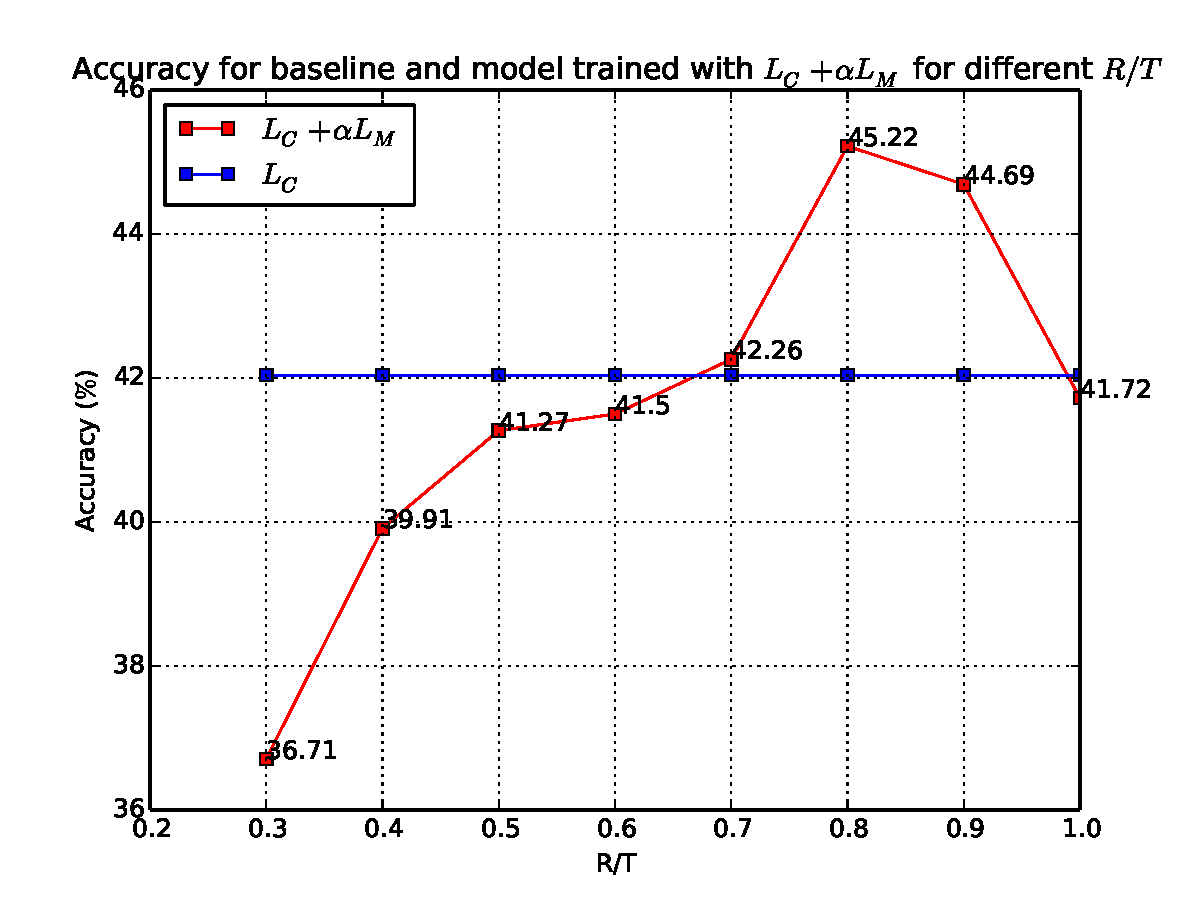
\includegraphics[scale=0.35]{accuracies.pdf}
	~
		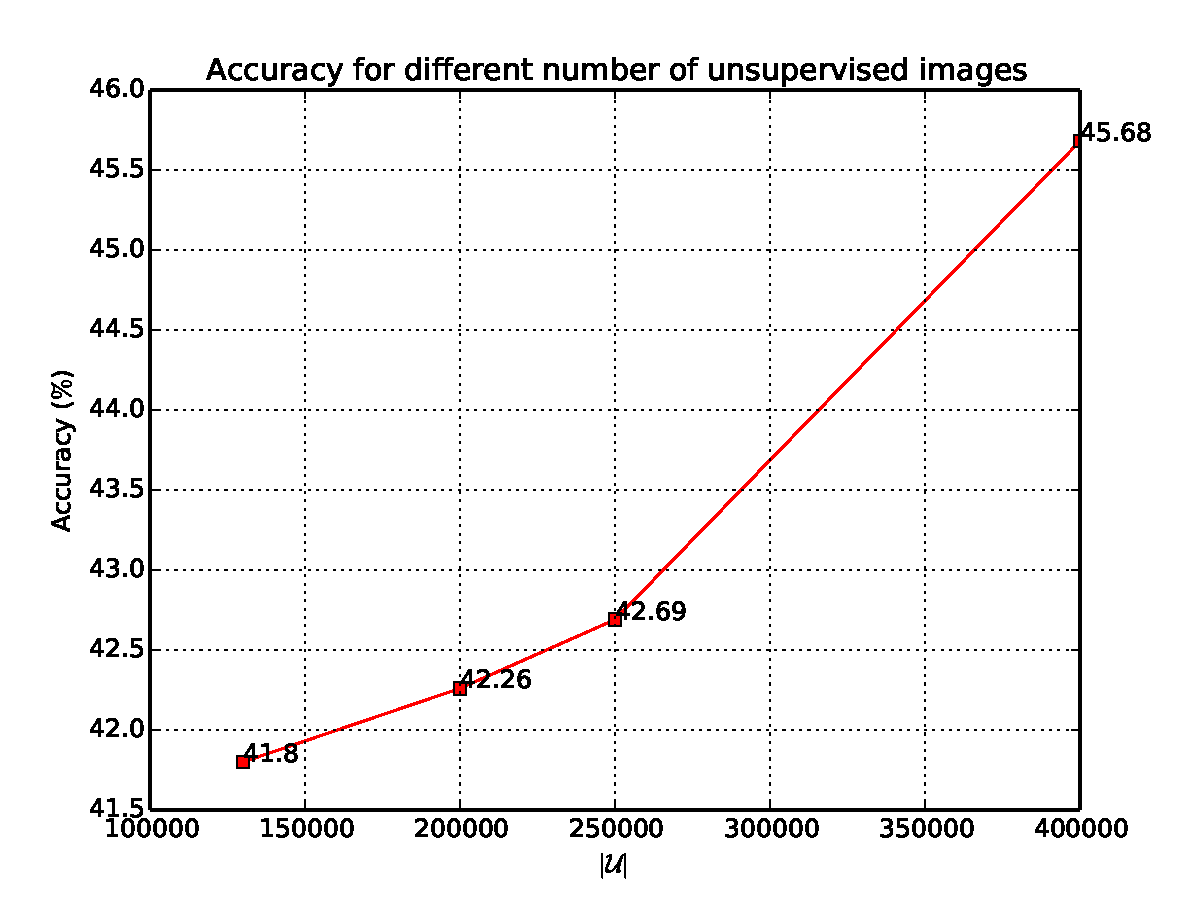
\includegraphics[scale=0.35]{accuracies_unsup.pdf}
	}
		\caption{(Left) Accuracy on the ImageNet validation set for models trained with the cross-entropy
		loss and MEL with $\mathcal{S}\cup\mathcal{U}$ (red) and only cross-entropy loss with
	$\mathcal{S}$ (blue). (Right) Accuracy of models trained with cross-entropy loss and MEL with
$\mathcal{S}\cup\mathcal{U}$ for $\frac{R}{T} = 0.7$ for different number of unsupervised images.}
		\label{fig:acc}
\end{figure}

Next, we vary the number of unsupervised images in the training set. Figure \ref{fig:acc} (right)
shows the validation accuracy for different amount of unsupervised data. We notice that more
unsupervised data is helpful for improving the classification performance. 

\subsection{Cross-entropy + MEL + NBEL}
Now we add the negative batch-entropy loss to cross-entropy loss and MEL. We vary $\beta$ while
keeping $\alpha$ and $\frac{R}{T}$ fixed from the previous case. The performance (accuracy on the
validation set) of these models hasn't reached the level of the previous cases. We
believe that this is because of the small batch sizes that we are using. Our next steps for this are
to increase the batch-size by using more GPUs or accumulating gradients over a few iterations before
updating the parameters.

\subsection{Cross-entropy + Loc}
In this case, we take the class activation map (CAM) of the class with the highest probability and
apply the locality penalty to this CAM. We have observed that CAMs
are able to localize some objects, but we haven't analyzed whether this is because of the
formulation of CAMs or because of our loss function. We plan to see the evolution of the
activations as training progresses to see if the area covered by the activations is reducing and
whether the CAMs are becoming more accurate with more training. 

\subsection{Transfer Learning}
For a comparison with recent work on unsupervised learning, we will experiment
with the transfer learning setting too. In this setting, models trained with only unsupervised
losses are used as initializations for other tasks (e.g. object detection, semantic segmentation).
We want to compare the unsupervised losses used by these works against ours. We also want to see if
models trained with both supervised and unsupervised losses are better than models trained with only
unsupervised losses for transfer learning. 

\bibliographystyle{splncs04}
\bibliography{report}

\end{document}
